\documentclass[]{article}
\usepackage{lmodern}
\usepackage{amssymb,amsmath}
\usepackage{ifxetex,ifluatex}
\usepackage{fixltx2e} % provides \textsubscript
\ifnum 0\ifxetex 1\fi\ifluatex 1\fi=0 % if pdftex
  \usepackage[T1]{fontenc}
  \usepackage[utf8]{inputenc}
\else % if luatex or xelatex
  \ifxetex
    \usepackage{mathspec}
  \else
    \usepackage{fontspec}
  \fi
  \defaultfontfeatures{Ligatures=TeX,Scale=MatchLowercase}
\fi
% use upquote if available, for straight quotes in verbatim environments
\IfFileExists{upquote.sty}{\usepackage{upquote}}{}
% use microtype if available
\IfFileExists{microtype.sty}{%
\usepackage[]{microtype}
\UseMicrotypeSet[protrusion]{basicmath} % disable protrusion for tt fonts
}{}
\PassOptionsToPackage{hyphens}{url} % url is loaded by hyperref
\usepackage[unicode=true]{hyperref}
\hypersetup{
            pdftitle={Hw4},
            pdfauthor={Calvin Wong},
            pdfborder={0 0 0},
            breaklinks=true}
\urlstyle{same}  % don't use monospace font for urls
\usepackage[margin=1in]{geometry}
\usepackage{color}
\usepackage{fancyvrb}
\newcommand{\VerbBar}{|}
\newcommand{\VERB}{\Verb[commandchars=\\\{\}]}
\DefineVerbatimEnvironment{Highlighting}{Verbatim}{commandchars=\\\{\}}
% Add ',fontsize=\small' for more characters per line
\usepackage{framed}
\definecolor{shadecolor}{RGB}{248,248,248}
\newenvironment{Shaded}{\begin{snugshade}}{\end{snugshade}}
\newcommand{\KeywordTok}[1]{\textcolor[rgb]{0.13,0.29,0.53}{\textbf{#1}}}
\newcommand{\DataTypeTok}[1]{\textcolor[rgb]{0.13,0.29,0.53}{#1}}
\newcommand{\DecValTok}[1]{\textcolor[rgb]{0.00,0.00,0.81}{#1}}
\newcommand{\BaseNTok}[1]{\textcolor[rgb]{0.00,0.00,0.81}{#1}}
\newcommand{\FloatTok}[1]{\textcolor[rgb]{0.00,0.00,0.81}{#1}}
\newcommand{\ConstantTok}[1]{\textcolor[rgb]{0.00,0.00,0.00}{#1}}
\newcommand{\CharTok}[1]{\textcolor[rgb]{0.31,0.60,0.02}{#1}}
\newcommand{\SpecialCharTok}[1]{\textcolor[rgb]{0.00,0.00,0.00}{#1}}
\newcommand{\StringTok}[1]{\textcolor[rgb]{0.31,0.60,0.02}{#1}}
\newcommand{\VerbatimStringTok}[1]{\textcolor[rgb]{0.31,0.60,0.02}{#1}}
\newcommand{\SpecialStringTok}[1]{\textcolor[rgb]{0.31,0.60,0.02}{#1}}
\newcommand{\ImportTok}[1]{#1}
\newcommand{\CommentTok}[1]{\textcolor[rgb]{0.56,0.35,0.01}{\textit{#1}}}
\newcommand{\DocumentationTok}[1]{\textcolor[rgb]{0.56,0.35,0.01}{\textbf{\textit{#1}}}}
\newcommand{\AnnotationTok}[1]{\textcolor[rgb]{0.56,0.35,0.01}{\textbf{\textit{#1}}}}
\newcommand{\CommentVarTok}[1]{\textcolor[rgb]{0.56,0.35,0.01}{\textbf{\textit{#1}}}}
\newcommand{\OtherTok}[1]{\textcolor[rgb]{0.56,0.35,0.01}{#1}}
\newcommand{\FunctionTok}[1]{\textcolor[rgb]{0.00,0.00,0.00}{#1}}
\newcommand{\VariableTok}[1]{\textcolor[rgb]{0.00,0.00,0.00}{#1}}
\newcommand{\ControlFlowTok}[1]{\textcolor[rgb]{0.13,0.29,0.53}{\textbf{#1}}}
\newcommand{\OperatorTok}[1]{\textcolor[rgb]{0.81,0.36,0.00}{\textbf{#1}}}
\newcommand{\BuiltInTok}[1]{#1}
\newcommand{\ExtensionTok}[1]{#1}
\newcommand{\PreprocessorTok}[1]{\textcolor[rgb]{0.56,0.35,0.01}{\textit{#1}}}
\newcommand{\AttributeTok}[1]{\textcolor[rgb]{0.77,0.63,0.00}{#1}}
\newcommand{\RegionMarkerTok}[1]{#1}
\newcommand{\InformationTok}[1]{\textcolor[rgb]{0.56,0.35,0.01}{\textbf{\textit{#1}}}}
\newcommand{\WarningTok}[1]{\textcolor[rgb]{0.56,0.35,0.01}{\textbf{\textit{#1}}}}
\newcommand{\AlertTok}[1]{\textcolor[rgb]{0.94,0.16,0.16}{#1}}
\newcommand{\ErrorTok}[1]{\textcolor[rgb]{0.64,0.00,0.00}{\textbf{#1}}}
\newcommand{\NormalTok}[1]{#1}
\usepackage{graphicx,grffile}
\makeatletter
\def\maxwidth{\ifdim\Gin@nat@width>\linewidth\linewidth\else\Gin@nat@width\fi}
\def\maxheight{\ifdim\Gin@nat@height>\textheight\textheight\else\Gin@nat@height\fi}
\makeatother
% Scale images if necessary, so that they will not overflow the page
% margins by default, and it is still possible to overwrite the defaults
% using explicit options in \includegraphics[width, height, ...]{}
\setkeys{Gin}{width=\maxwidth,height=\maxheight,keepaspectratio}
\IfFileExists{parskip.sty}{%
\usepackage{parskip}
}{% else
\setlength{\parindent}{0pt}
\setlength{\parskip}{6pt plus 2pt minus 1pt}
}
\setlength{\emergencystretch}{3em}  % prevent overfull lines
\providecommand{\tightlist}{%
  \setlength{\itemsep}{0pt}\setlength{\parskip}{0pt}}
\setcounter{secnumdepth}{0}
% Redefines (sub)paragraphs to behave more like sections
\ifx\paragraph\undefined\else
\let\oldparagraph\paragraph
\renewcommand{\paragraph}[1]{\oldparagraph{#1}\mbox{}}
\fi
\ifx\subparagraph\undefined\else
\let\oldsubparagraph\subparagraph
\renewcommand{\subparagraph}[1]{\oldsubparagraph{#1}\mbox{}}
\fi

% set default figure placement to htbp
\makeatletter
\def\fps@figure{htbp}
\makeatother


\title{Hw4}
\author{Calvin Wong}
\date{2/28/2020}

\begin{document}
\maketitle

\begin{Shaded}
\begin{Highlighting}[]
\KeywordTok{library}\NormalTok{(fpp2)}
\end{Highlighting}
\end{Shaded}

\begin{verbatim}
## Loading required package: ggplot2
\end{verbatim}

\begin{verbatim}
## Warning: package 'ggplot2' was built under R version 3.5.2
\end{verbatim}

\begin{verbatim}
## Loading required package: forecast
\end{verbatim}

\begin{verbatim}
## Warning: package 'forecast' was built under R version 3.5.2
\end{verbatim}

\begin{verbatim}
## Loading required package: fma
\end{verbatim}

\begin{verbatim}
## Warning: package 'fma' was built under R version 3.5.2
\end{verbatim}

\begin{verbatim}
## Loading required package: expsmooth
\end{verbatim}

\begin{Shaded}
\begin{Highlighting}[]
\KeywordTok{library}\NormalTok{(forecast)}
\KeywordTok{library}\NormalTok{(seasonal)}
\KeywordTok{library}\NormalTok{(gridExtra)}
\end{Highlighting}
\end{Shaded}

\begin{enumerate}
\def\labelenumi{\arabic{enumi}.}
\tightlist
\item
  Consider the pigs series --- the number of pigs slaughtered in
  Victoria each month.
\end{enumerate}

\begin{enumerate}
\def\labelenumi{\alph{enumi})}
\tightlist
\item
  Use the ses() function in R to find the optimal values of α and ℓ0,
  and generate forecasts for the next four months.
\end{enumerate}

α = 0.2971 ℓ0 = 10308.58

\begin{Shaded}
\begin{Highlighting}[]
\KeywordTok{summary}\NormalTok{(}\KeywordTok{ses}\NormalTok{(pigs,}\DataTypeTok{h=}\DecValTok{4}\NormalTok{))}
\end{Highlighting}
\end{Shaded}

\begin{verbatim}
## 
## Forecast method: Simple exponential smoothing
## 
## Model Information:
## Simple exponential smoothing 
## 
## Call:
##  ses(y = pigs, h = 4) 
## 
##   Smoothing parameters:
##     alpha = 0.2971 
## 
##   Initial states:
##     l = 77260.0561 
## 
##   sigma:  10308.58
## 
##      AIC     AICc      BIC 
## 4462.955 4463.086 4472.665 
## 
## Error measures:
##                    ME    RMSE      MAE       MPE     MAPE      MASE       ACF1
## Training set 385.8721 10253.6 7961.383 -0.922652 9.274016 0.7966249 0.01282239
## 
## Forecasts:
##          Point Forecast    Lo 80    Hi 80    Lo 95    Hi 95
## Sep 1995       98816.41 85605.43 112027.4 78611.97 119020.8
## Oct 1995       98816.41 85034.52 112598.3 77738.83 119894.0
## Nov 1995       98816.41 84486.34 113146.5 76900.46 120732.4
## Dec 1995       98816.41 83958.37 113674.4 76092.99 121539.8
\end{verbatim}

\begin{enumerate}
\def\labelenumi{\alph{enumi})}
\setcounter{enumi}{1}
\tightlist
\item
  Compute a 95\% prediction interval for the first forecast using \^{}y
  ± 1.96s where s is the standard deviation of the residuals. Compare
  your interval with the interval produced by R.
\end{enumerate}

\begin{Shaded}
\begin{Highlighting}[]
\NormalTok{s<-}\KeywordTok{sd}\NormalTok{((}\KeywordTok{ses}\NormalTok{(pigs, }\DataTypeTok{h=}\DecValTok{4}\NormalTok{))}\OperatorTok{$}\NormalTok{residuals)}
\NormalTok{s}
\end{Highlighting}
\end{Shaded}

\begin{verbatim}
## [1] 10273.69
\end{verbatim}

\begin{Shaded}
\begin{Highlighting}[]
\KeywordTok{ses}\NormalTok{(pigs,}\DataTypeTok{h=}\DecValTok{4}\NormalTok{)}\OperatorTok{$}\NormalTok{mean[}\DecValTok{1}\NormalTok{]}\OperatorTok{+}\FloatTok{1.96}\OperatorTok{*}\NormalTok{s}
\end{Highlighting}
\end{Shaded}

\begin{verbatim}
## [1] 118952.8
\end{verbatim}

\begin{enumerate}
\def\labelenumi{\arabic{enumi}.}
\setcounter{enumi}{4}
\tightlist
\item
  Data set books contains the daily sales of paperback and hardcover
  books at the same store. The task is to forecast the next four days'
  sales for paperback and hardcover books.
\end{enumerate}

\begin{enumerate}
\def\labelenumi{\alph{enumi})}
\tightlist
\item
  Plot the series and discuss the main features of the data.
\end{enumerate}

\begin{Shaded}
\begin{Highlighting}[]
\KeywordTok{autoplot}\NormalTok{(books) }\OperatorTok{+}\StringTok{ }\KeywordTok{xlab}\NormalTok{(}\StringTok{"Day"}\NormalTok{)}
\end{Highlighting}
\end{Shaded}

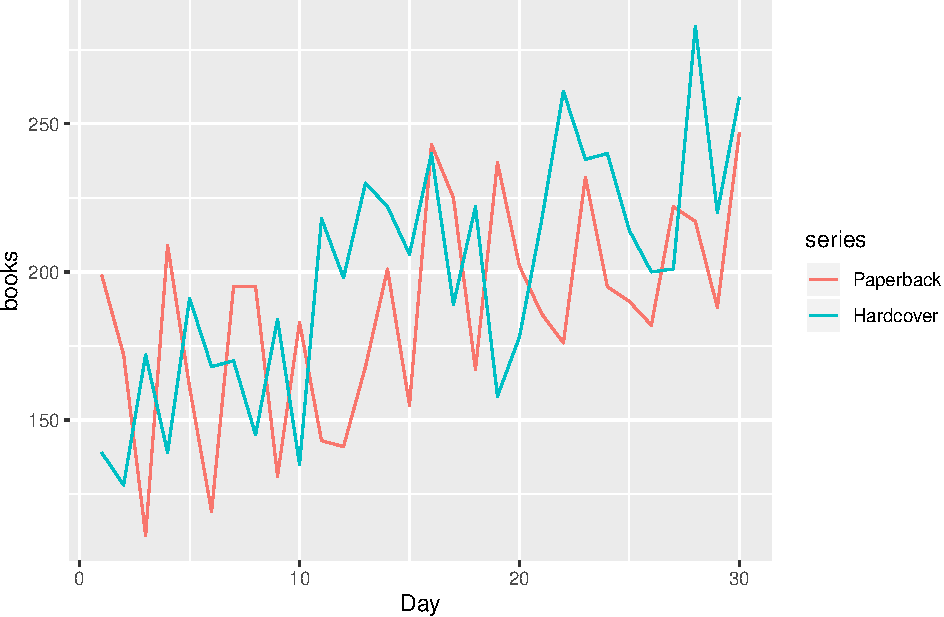
\includegraphics{Hw4_files/figure-latex/unnamed-chunk-5-1.pdf}

\begin{enumerate}
\def\labelenumi{\alph{enumi})}
\setcounter{enumi}{1}
\tightlist
\item
  Use the ses() function to forecast each series, and plot the
  forecasts.
\end{enumerate}

\begin{Shaded}
\begin{Highlighting}[]
\NormalTok{sespb <-}\StringTok{ }\KeywordTok{ses}\NormalTok{(books[,}\DecValTok{1}\NormalTok{])}
\NormalTok{seshc <-}\StringTok{ }\KeywordTok{ses}\NormalTok{(books[,}\DecValTok{2}\NormalTok{])}

\NormalTok{pb1 <-}\StringTok{ }\KeywordTok{autoplot}\NormalTok{(sespb) }\OperatorTok{+}
\StringTok{  }\KeywordTok{autolayer}\NormalTok{(}\KeywordTok{fitted}\NormalTok{(sespb), }\DataTypeTok{series=}\StringTok{'Fitted'}\NormalTok{) }\OperatorTok{+}
\StringTok{  }\KeywordTok{ggtitle}\NormalTok{(}\StringTok{'SES Paperback Sale Forecast'}\NormalTok{) }\OperatorTok{+}
\StringTok{  }\KeywordTok{xlab}\NormalTok{(}\StringTok{'Day'}\NormalTok{) }\OperatorTok{+}
\StringTok{  }\KeywordTok{ylab}\NormalTok{(}\StringTok{'Books'}\NormalTok{)}
\NormalTok{pb1}
\end{Highlighting}
\end{Shaded}

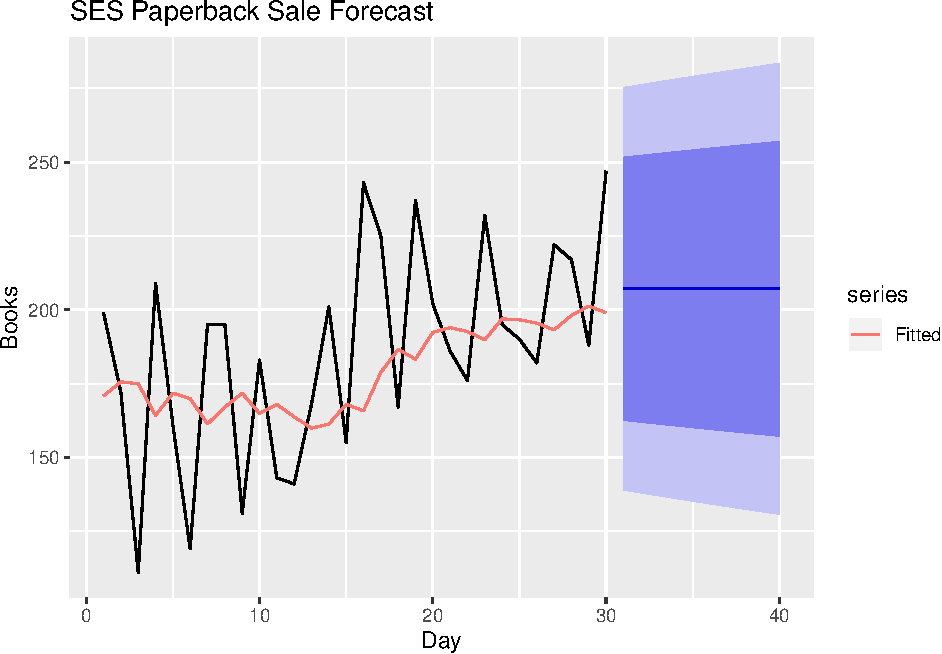
\includegraphics{Hw4_files/figure-latex/unnamed-chunk-6-1.pdf}

\begin{Shaded}
\begin{Highlighting}[]
\NormalTok{hc1 <-}\StringTok{ }\KeywordTok{autoplot}\NormalTok{(seshc) }\OperatorTok{+}
\StringTok{  }\KeywordTok{autolayer}\NormalTok{(}\KeywordTok{fitted}\NormalTok{(seshc), }\DataTypeTok{series=}\StringTok{'Fitted'}\NormalTok{) }\OperatorTok{+}
\StringTok{  }\KeywordTok{ggtitle}\NormalTok{(}\StringTok{'SES Hardcover Sale Forecast'}\NormalTok{) }\OperatorTok{+}
\StringTok{  }\KeywordTok{xlab}\NormalTok{(}\StringTok{'Day'}\NormalTok{) }\OperatorTok{+}
\StringTok{  }\KeywordTok{ylab}\NormalTok{(}\StringTok{'Books'}\NormalTok{)}
\NormalTok{hc1}
\end{Highlighting}
\end{Shaded}

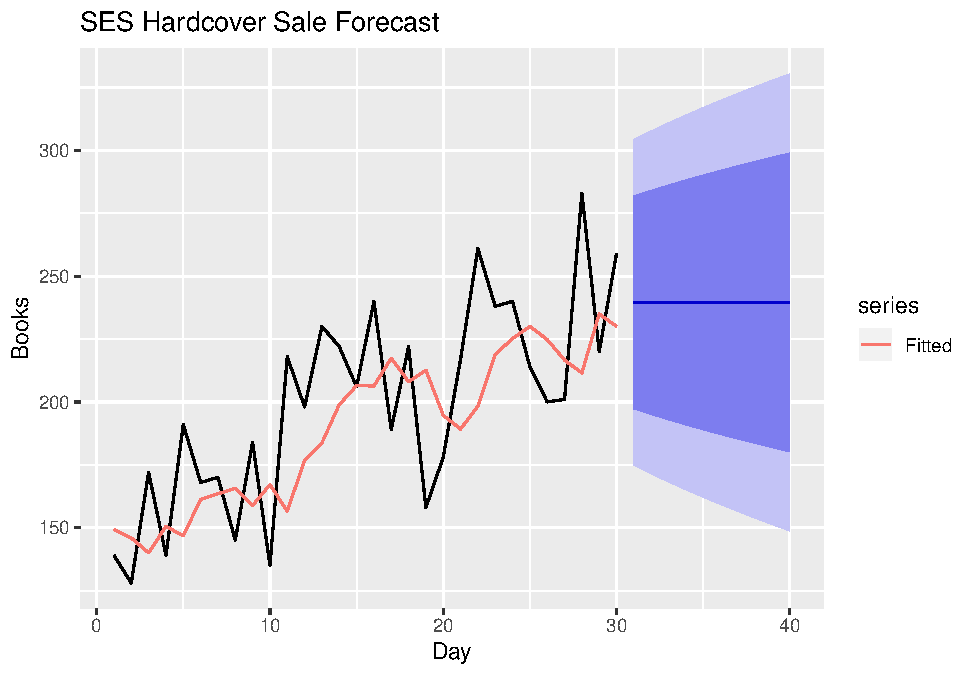
\includegraphics{Hw4_files/figure-latex/unnamed-chunk-6-2.pdf}

\begin{enumerate}
\def\labelenumi{\alph{enumi})}
\setcounter{enumi}{2}
\tightlist
\item
  Compute the RMSE values for the training data in each case.
\end{enumerate}

\begin{Shaded}
\begin{Highlighting}[]
\KeywordTok{round}\NormalTok{(}\KeywordTok{accuracy}\NormalTok{(sespb), }\DecValTok{2}\NormalTok{)}
\end{Highlighting}
\end{Shaded}

\begin{verbatim}
##                ME  RMSE   MAE  MPE  MAPE MASE  ACF1
## Training set 7.18 33.64 27.84 0.47 15.58  0.7 -0.21
\end{verbatim}

\begin{Shaded}
\begin{Highlighting}[]
\KeywordTok{round}\NormalTok{(}\KeywordTok{accuracy}\NormalTok{(seshc), }\DecValTok{2}\NormalTok{)}
\end{Highlighting}
\end{Shaded}

\begin{verbatim}
##                ME  RMSE   MAE  MPE  MAPE MASE  ACF1
## Training set 9.17 31.93 26.77 2.64 13.39  0.8 -0.14
\end{verbatim}

\begin{enumerate}
\def\labelenumi{\arabic{enumi}.}
\setcounter{enumi}{5}
\tightlist
\item
  We will continue with the daily sales of paperback and hardcover books
  in data set books.
\end{enumerate}

\begin{enumerate}
\def\labelenumi{\alph{enumi})}
\tightlist
\item
  Apply Holt's linear method to the paperback and hardback series and
  compute four-day forecasts in each case.
\end{enumerate}

\begin{Shaded}
\begin{Highlighting}[]
\NormalTok{holtpb <-}\StringTok{ }\KeywordTok{holt}\NormalTok{(books[,}\DecValTok{1}\NormalTok{], }\DataTypeTok{h=}\DecValTok{4}\NormalTok{)}
\KeywordTok{forecast}\NormalTok{(holtpb)}
\end{Highlighting}
\end{Shaded}

\begin{verbatim}
##    Point Forecast    Lo 80    Hi 80    Lo 95    Hi 95
## 31       209.4668 166.6035 252.3301 143.9130 275.0205
## 32       210.7177 167.8544 253.5811 145.1640 276.2715
## 33       211.9687 169.1054 254.8320 146.4149 277.5225
## 34       213.2197 170.3564 256.0830 147.6659 278.7735
\end{verbatim}

\begin{Shaded}
\begin{Highlighting}[]
\NormalTok{holthc <-}\StringTok{ }\KeywordTok{holt}\NormalTok{(books[,}\DecValTok{2}\NormalTok{], }\DataTypeTok{h=}\DecValTok{4}\NormalTok{)}
\KeywordTok{forecast}\NormalTok{(holthc)}
\end{Highlighting}
\end{Shaded}

\begin{verbatim}
##    Point Forecast    Lo 80    Hi 80    Lo 95    Hi 95
## 31       250.1739 212.7390 287.6087 192.9222 307.4256
## 32       253.4765 216.0416 290.9113 196.2248 310.7282
## 33       256.7791 219.3442 294.2140 199.5274 314.0308
## 34       260.0817 222.6468 297.5166 202.8300 317.3334
\end{verbatim}

\begin{enumerate}
\def\labelenumi{\alph{enumi})}
\setcounter{enumi}{1}
\tightlist
\item
  Compare the RMSE measures of Holt's method for the two series to those
  of simple exponential smoothing in the previous question. (Remember
  that Holt's method is using one more parameter than SES.) Discuss the
  merits of the two forecasting methods for these data sets.
\end{enumerate}

\begin{Shaded}
\begin{Highlighting}[]
\KeywordTok{round}\NormalTok{(}\KeywordTok{accuracy}\NormalTok{(holtpb), }\DecValTok{2}\NormalTok{)}
\end{Highlighting}
\end{Shaded}

\begin{verbatim}
##                 ME  RMSE   MAE   MPE  MAPE MASE  ACF1
## Training set -3.72 31.14 26.18 -5.51 15.58 0.66 -0.18
\end{verbatim}

\begin{Shaded}
\begin{Highlighting}[]
\KeywordTok{round}\NormalTok{(}\KeywordTok{accuracy}\NormalTok{(holthc), }\DecValTok{2}\NormalTok{)}
\end{Highlighting}
\end{Shaded}

\begin{verbatim}
##                 ME  RMSE   MAE   MPE  MAPE MASE  ACF1
## Training set -0.14 27.19 23.16 -2.11 12.16 0.69 -0.03
\end{verbatim}

\begin{enumerate}
\def\labelenumi{\alph{enumi})}
\setcounter{enumi}{2}
\tightlist
\item
  Compare the forecasts for the two series using both methods. Which do
  you think is best?
\end{enumerate}

\begin{Shaded}
\begin{Highlighting}[]
\NormalTok{pb2 <-}\StringTok{ }\KeywordTok{autoplot}\NormalTok{(holtpb) }\OperatorTok{+}
\StringTok{  }\KeywordTok{autolayer}\NormalTok{(}\KeywordTok{fitted}\NormalTok{(sespb), }\DataTypeTok{series =} \StringTok{"Pred. Paperback"}\NormalTok{) }\OperatorTok{+}\StringTok{ }
\StringTok{  }\KeywordTok{xlab}\NormalTok{(}\StringTok{"Time"}\NormalTok{) }\OperatorTok{+}\StringTok{ }\KeywordTok{ylab}\NormalTok{(}\StringTok{"Books"}\NormalTok{)}
\KeywordTok{grid.arrange}\NormalTok{(pb1,pb2)}
\end{Highlighting}
\end{Shaded}

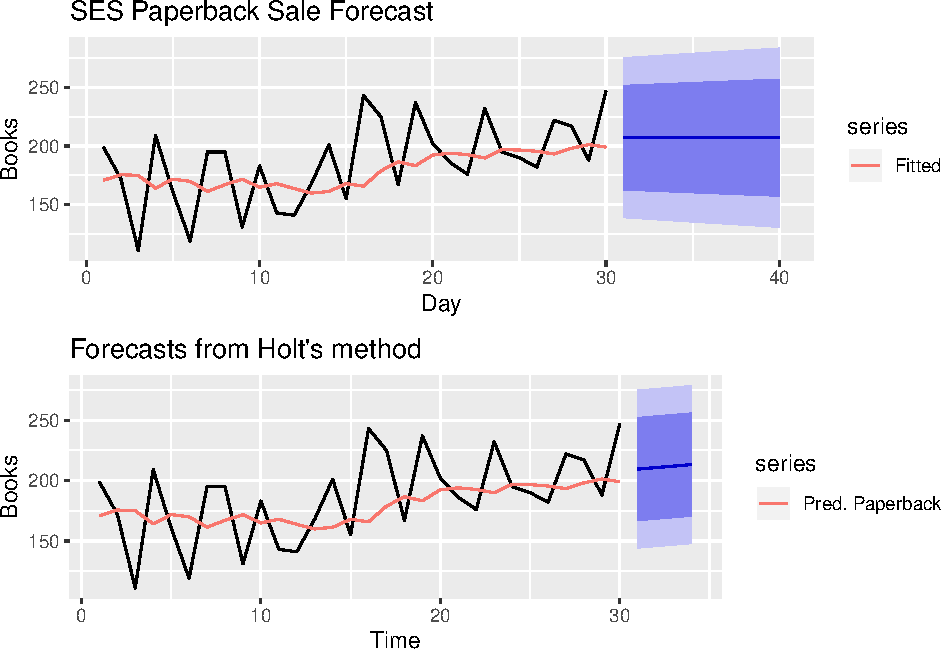
\includegraphics{Hw4_files/figure-latex/unnamed-chunk-13-1.pdf}

\begin{Shaded}
\begin{Highlighting}[]
\NormalTok{hc2 <-}\StringTok{ }\KeywordTok{autoplot}\NormalTok{(holthc) }\OperatorTok{+}
\StringTok{  }\KeywordTok{autolayer}\NormalTok{(}\KeywordTok{fitted}\NormalTok{(seshc), }\DataTypeTok{series =} \StringTok{"Pred. Hardcover"}\NormalTok{) }\OperatorTok{+}
\StringTok{  }\KeywordTok{xlab}\NormalTok{(}\StringTok{"Time"}\NormalTok{) }\OperatorTok{+}\StringTok{ }\KeywordTok{ylab}\NormalTok{(}\StringTok{"Sales"}\NormalTok{)}

\KeywordTok{grid.arrange}\NormalTok{(hc1,hc2)}
\end{Highlighting}
\end{Shaded}

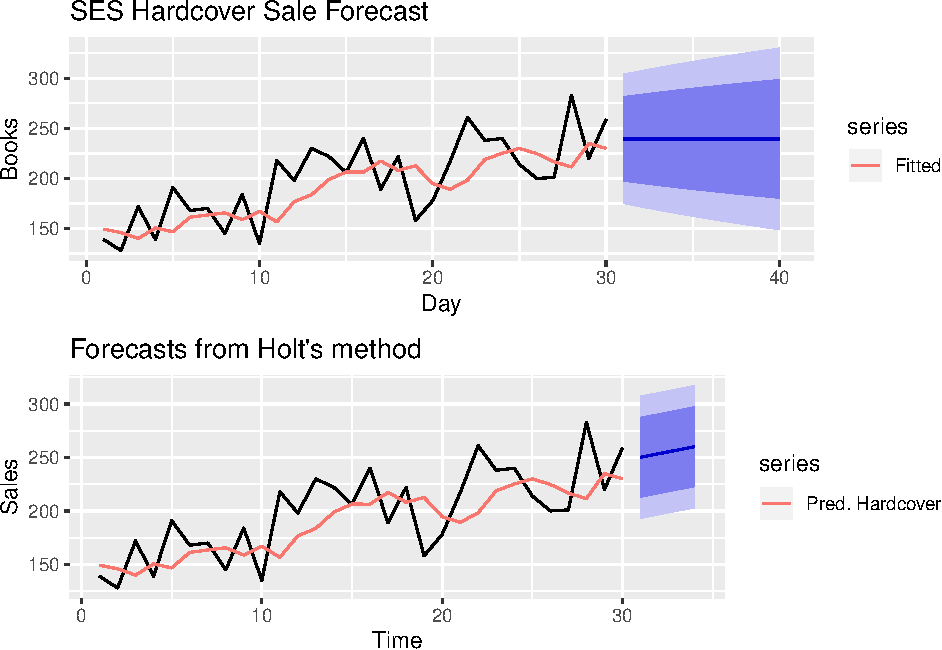
\includegraphics{Hw4_files/figure-latex/unnamed-chunk-14-1.pdf}

Comparing both models, in terms of RMSE, holt is the best model. In
terms of fitted plot, holt outperforms the hardcover, however if we look
at the paperback in case of holt method the forecast does not seems to
represent the actual series, which is a little concerning in an attempt
to choose the best model.

\begin{enumerate}
\def\labelenumi{\alph{enumi})}
\setcounter{enumi}{3}
\tightlist
\item
  Calculate a 95\% prediction interval for the first forecast for each
  series, using the RMSE values and assuming normal errors. Compare your
  intervals with those produced using ses and holt.
\end{enumerate}

\begin{enumerate}
\def\labelenumi{\arabic{enumi}.}
\setcounter{enumi}{6}
\tightlist
\item
  For this exercise use data set eggs, the price of a dozen eggs in the
  United States from 1900--1993. Experiment with the various options in
  the holt() function to see how much the forecasts change with damped
  trend, or with a Box-Cox transformation. Try to develop an intuition
  of what each argument is doing to the forecasts.
\end{enumerate}

{[}Hint: use h=100 when calling holt() so you can clearly see the
differences between the various options when plotting the forecasts.{]}
Which model gives the best RMSE?

\begin{Shaded}
\begin{Highlighting}[]
\NormalTok{holt_r <-}\StringTok{ }\KeywordTok{holt}\NormalTok{(eggs,}\DataTypeTok{h=}\DecValTok{100}\NormalTok{)}
\NormalTok{holt_damped<-}\KeywordTok{holt}\NormalTok{(eggs,}\DataTypeTok{damped =} \OtherTok{TRUE}\NormalTok{,}\DataTypeTok{h=}\DecValTok{100}\NormalTok{)}
\NormalTok{holt_bc <-}\KeywordTok{holt}\NormalTok{(eggs, }\DataTypeTok{lambda=}\KeywordTok{BoxCox.lambda}\NormalTok{(eggs),}\DataTypeTok{h=}\DecValTok{100}\NormalTok{)}

\NormalTok{a1 <-}\StringTok{ }\KeywordTok{autoplot}\NormalTok{(holt_r)}
\NormalTok{a2 <-}\StringTok{ }\KeywordTok{autoplot}\NormalTok{(holt_damped)}
\NormalTok{a3 <-}\StringTok{ }\KeywordTok{autoplot}\NormalTok{(holt_bc)}

\KeywordTok{grid.arrange}\NormalTok{(a1, a2, a3, }\DataTypeTok{ncol=}\DecValTok{2}\NormalTok{)}
\end{Highlighting}
\end{Shaded}

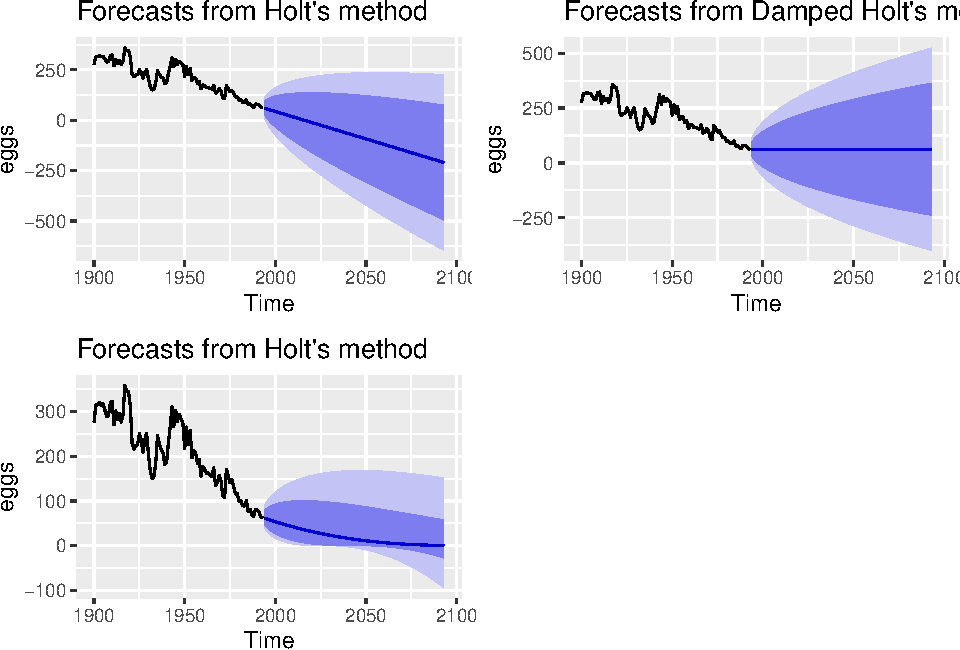
\includegraphics{Hw4_files/figure-latex/unnamed-chunk-16-1.pdf}

\begin{Shaded}
\begin{Highlighting}[]
\KeywordTok{accuracy}\NormalTok{(holt_r)}
\end{Highlighting}
\end{Shaded}

\begin{verbatim}
##                      ME     RMSE      MAE       MPE     MAPE      MASE
## Training set 0.04499087 26.58219 19.18491 -1.142201 9.653791 0.9463626
##                    ACF1
## Training set 0.01348202
\end{verbatim}

\begin{Shaded}
\begin{Highlighting}[]
\KeywordTok{accuracy}\NormalTok{(holt_damped)}
\end{Highlighting}
\end{Shaded}

\begin{verbatim}
##                     ME     RMSE     MAE       MPE     MAPE      MASE
## Training set -2.891496 26.54019 19.2795 -2.907633 10.01894 0.9510287
##                      ACF1
## Training set -0.003195358
\end{verbatim}

\begin{Shaded}
\begin{Highlighting}[]
\KeywordTok{accuracy}\NormalTok{(holt_bc)}
\end{Highlighting}
\end{Shaded}

\begin{verbatim}
##                     ME     RMSE      MAE       MPE     MAPE      MASE
## Training set 0.7736844 26.39376 18.96387 -1.072416 9.620095 0.9354593
##                    ACF1
## Training set 0.03887152
\end{verbatim}

Comparing the accuracy of the three models reveal that the RMSE scores
were similar, however holt with box-cox has a slight edge among the
different methods. Therefore, holt with boxcox will be the best model
for this example.

\begin{enumerate}
\def\labelenumi{\arabic{enumi}.}
\setcounter{enumi}{7}
\tightlist
\item
  Recall your retail time series data (from Exercise 3 in Section 2.10).
\end{enumerate}

\begin{Shaded}
\begin{Highlighting}[]
\NormalTok{retaildata <-}\StringTok{ }\NormalTok{readxl}\OperatorTok{::}\KeywordTok{read_excel}\NormalTok{(}\StringTok{"retail.xlsx"}\NormalTok{, }\DataTypeTok{skip=}\DecValTok{1}\NormalTok{)}
\NormalTok{myts <-}\StringTok{ }\KeywordTok{ts}\NormalTok{(retaildata[,}\StringTok{"A3349909T"}\NormalTok{], }\DataTypeTok{frequency=}\DecValTok{12}\NormalTok{, }\DataTypeTok{start=}\KeywordTok{c}\NormalTok{(}\DecValTok{1982}\NormalTok{,}\DecValTok{4}\NormalTok{))}
\KeywordTok{autoplot}\NormalTok{(myts)}
\end{Highlighting}
\end{Shaded}

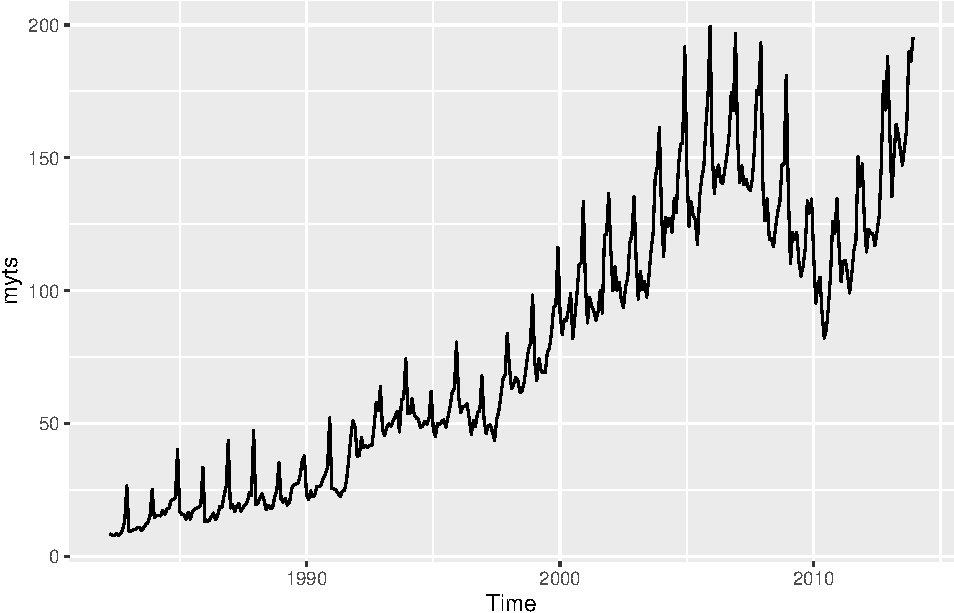
\includegraphics{Hw4_files/figure-latex/unnamed-chunk-18-1.pdf}

\begin{enumerate}
\def\labelenumi{\alph{enumi})}
\tightlist
\item
  Why is multiplicative seasonality necessary for this series?
\end{enumerate}

It is clear from the graph that seasonality variations are changing with
increase in time. In that case, multiplicative seasonality is the best
approach because seasonal variations are not constant and additive
method can handle constant seasonal variations only.

\begin{enumerate}
\def\labelenumi{\alph{enumi})}
\setcounter{enumi}{1}
\tightlist
\item
  Apply Holt-Winters' multiplicative method to the data. Experiment with
  making the trend damped.
\end{enumerate}

\begin{Shaded}
\begin{Highlighting}[]
\NormalTok{hw_myts <-}\StringTok{ }\KeywordTok{hw}\NormalTok{(myts, }\DataTypeTok{seasonal =} \StringTok{"multiplicative"}\NormalTok{, }\DataTypeTok{h=}\DecValTok{100}\NormalTok{)}
\NormalTok{hw_myts_damped  <-}\StringTok{ }\KeywordTok{hw}\NormalTok{(myts, }\DataTypeTok{damped =}\OtherTok{TRUE}\NormalTok{, }\DataTypeTok{seasonal =} \StringTok{"multiplicative"}\NormalTok{, }\DataTypeTok{h=}\DecValTok{100}\NormalTok{)}

\KeywordTok{autoplot}\NormalTok{(myts) }\OperatorTok{+}\StringTok{ }\KeywordTok{autolayer}\NormalTok{(hw_myts, }\DataTypeTok{series=}\StringTok{'Retail Data Multiplicative'}\NormalTok{, }\DataTypeTok{PI=}\OtherTok{FALSE}\NormalTok{)  }\OperatorTok{+}
\StringTok{    }\KeywordTok{autolayer}\NormalTok{(hw_myts_damped, }\DataTypeTok{series=}\StringTok{'Retail Data Damped'}\NormalTok{, }\DataTypeTok{PI=}\OtherTok{FALSE}\NormalTok{) }
\end{Highlighting}
\end{Shaded}

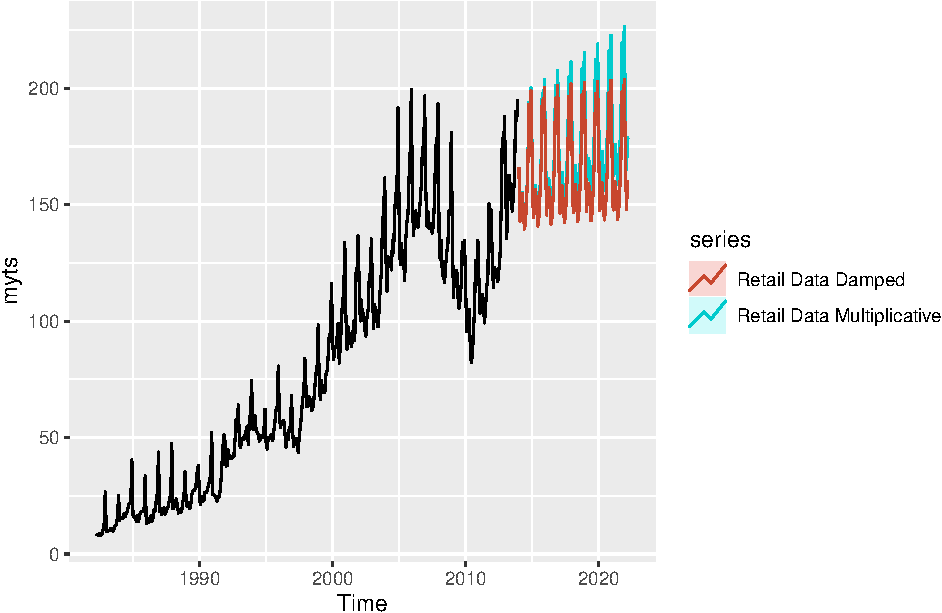
\includegraphics{Hw4_files/figure-latex/unnamed-chunk-19-1.pdf}

\begin{enumerate}
\def\labelenumi{\alph{enumi})}
\setcounter{enumi}{2}
\tightlist
\item
  Compare the RMSE of the one-step forecasts from the two methods. Which
  do you prefer?
\end{enumerate}

The RMSE values are very similiar. Because it takes the same amount of
effort to get either, I will go with the Holt-Winters' multiplicative
method.

\begin{Shaded}
\begin{Highlighting}[]
\NormalTok{os_hw <-}\StringTok{  }\KeywordTok{forecast}\NormalTok{(hw_myts, }\DataTypeTok{h=}\DecValTok{1}\NormalTok{)}
\KeywordTok{accuracy}\NormalTok{(os_hw)}
\end{Highlighting}
\end{Shaded}

\begin{verbatim}
##                     ME    RMSE      MAE        MPE     MAPE    MASE       ACF1
## Training set 0.1501056 5.13465 3.636702 -0.3051469 6.605764 0.37101 0.03047222
\end{verbatim}

\begin{Shaded}
\begin{Highlighting}[]
\NormalTok{os_hw_damped <-}\StringTok{ }\KeywordTok{forecast}\NormalTok{(hw_myts_damped, }\DataTypeTok{h=}\DecValTok{1}\NormalTok{)}
\KeywordTok{accuracy}\NormalTok{(os_hw_damped)}
\end{Highlighting}
\end{Shaded}

\begin{verbatim}
##                     ME     RMSE      MAE      MPE     MAPE      MASE       ACF1
## Training set 0.3846631 5.134439 3.640449 0.331356 6.605576 0.3713922 0.02482746
\end{verbatim}

\begin{enumerate}
\def\labelenumi{\alph{enumi})}
\setcounter{enumi}{3}
\tightlist
\item
  Check that the residuals from the best method look like white noise.
\end{enumerate}

\begin{Shaded}
\begin{Highlighting}[]
\KeywordTok{checkresiduals}\NormalTok{(hw_myts_damped)}
\end{Highlighting}
\end{Shaded}

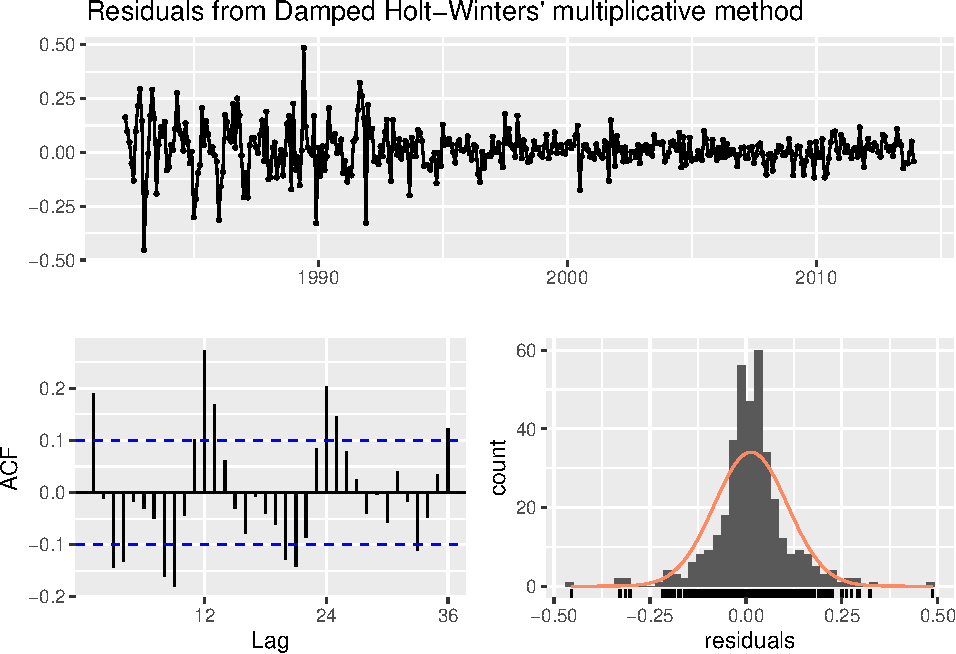
\includegraphics{Hw4_files/figure-latex/unnamed-chunk-22-1.pdf}

\begin{verbatim}
## 
##  Ljung-Box test
## 
## data:  Residuals from Damped Holt-Winters' multiplicative method
## Q* = 143, df = 7, p-value < 2.2e-16
## 
## Model df: 17.   Total lags used: 24
\end{verbatim}

\begin{enumerate}
\def\labelenumi{\alph{enumi})}
\setcounter{enumi}{4}
\tightlist
\item
  Now find the test set RMSE, while training the model to the end of
  2010. Can you beat the seasonal naïve approach from Exercise 8 in
  Section 3.7?
\end{enumerate}

No, naive model at 27.4879 and multiplicative at 27.5280. The results
are very close.

\begin{Shaded}
\begin{Highlighting}[]
\NormalTok{myts.train <-}\StringTok{ }\KeywordTok{window}\NormalTok{(myts, }\DataTypeTok{end=}\KeywordTok{c}\NormalTok{(}\DecValTok{2010}\NormalTok{,}\DecValTok{12}\NormalTok{))}
\NormalTok{myts.test <-}\StringTok{ }\KeywordTok{window}\NormalTok{(myts, }\DataTypeTok{start=}\DecValTok{2011}\NormalTok{)}
\NormalTok{fc <-}\StringTok{ }\KeywordTok{snaive}\NormalTok{(myts.train)}
\KeywordTok{accuracy}\NormalTok{(fc,myts.test)}
\end{Highlighting}
\end{Shaded}

\begin{verbatim}
##                     ME     RMSE       MAE       MPE     MAPE     MASE      ACF1
## Training set  3.388889 11.45467  8.768468  6.646756 13.88686 1.000000 0.8226344
## Test set     23.620833 27.48790 23.620833 17.658958 17.65896 2.693838 0.7694841
##              Theil's U
## Training set        NA
## Test set      2.051517
\end{verbatim}

\begin{Shaded}
\begin{Highlighting}[]
\NormalTok{mc <-}\StringTok{ }\KeywordTok{hw}\NormalTok{(myts.train, }\DataTypeTok{damped =} \OtherTok{TRUE}\NormalTok{, }\DataTypeTok{seasonal =} \StringTok{"multiplicative"}\NormalTok{)}
\KeywordTok{accuracy}\NormalTok{(mc, myts.test)}
\end{Highlighting}
\end{Shaded}

\begin{verbatim}
##                      ME      RMSE       MAE        MPE      MAPE      MASE
## Training set  0.2442447  4.908721  3.471049  0.3999632  6.995412 0.3958557
## Test set     23.4061198 27.528045 23.406120 17.1755088 17.175509 2.6693510
##                     ACF1 Theil's U
## Training set -0.02018865        NA
## Test set      0.76879637  1.979646
\end{verbatim}

\begin{enumerate}
\def\labelenumi{\arabic{enumi}.}
\setcounter{enumi}{8}
\tightlist
\item
  For the same retail data, try an STL decomposition applied to the
  Box-Cox transformed series, followed by ETS on the seasonally adjusted
  data. How does that compare with your best previous forecasts on the
  test set?
\end{enumerate}

By extracting seasonal adjusted data, the RMSE of ETS on seasonally
adjusted method was better than all the methods. I will select this
method.

\begin{Shaded}
\begin{Highlighting}[]
\NormalTok{bc <-}\StringTok{ }\KeywordTok{BoxCox.lambda}\NormalTok{(myts.train)}
\NormalTok{fc_bc<-}\KeywordTok{BoxCox}\NormalTok{(myts.train,bc)}
\NormalTok{stl_bc <-}\StringTok{ }\KeywordTok{stlm}\NormalTok{(fc_bc)}
\NormalTok{myts.bc <-}\StringTok{ }\KeywordTok{forecast}\NormalTok{(stl_bc)}
\KeywordTok{autoplot}\NormalTok{(myts.bc)}
\end{Highlighting}
\end{Shaded}

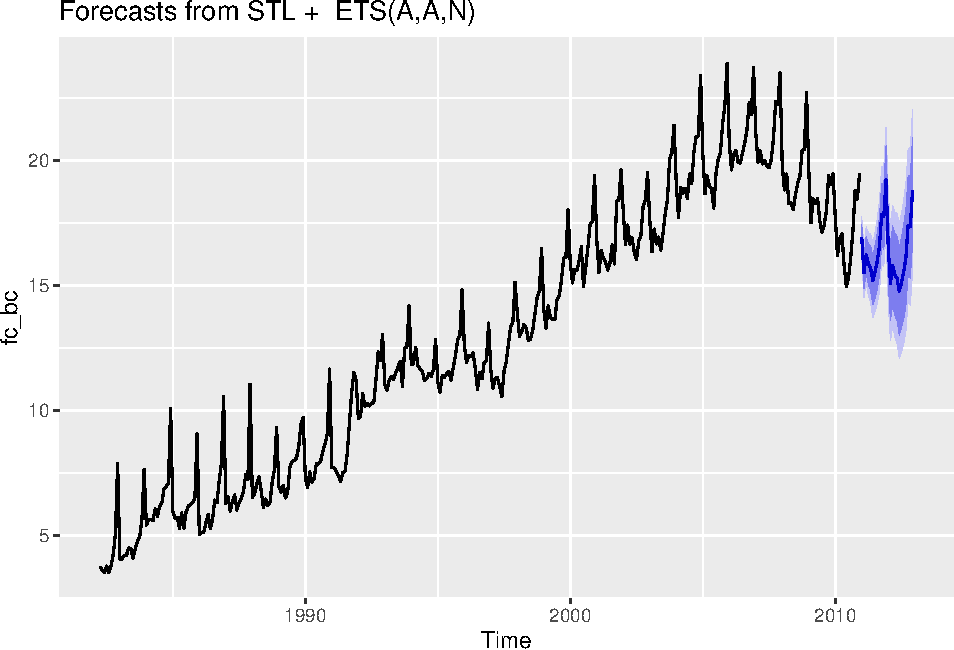
\includegraphics{Hw4_files/figure-latex/unnamed-chunk-24-1.pdf}

\end{document}
